%----------------------------------------------------------------------------------------
%	PACKAGES AND THEMES  (formatting taken from the 30-min presentation)
%----------------------------------------------------------------------------------------
\documentclass[aspectratio=169,xcolor=table]{beamer}

%-- Layout --%
\usepackage[fontsize=11pt]{scrextend}
\usepackage{amsmath}
\usepackage{amssymb}
\usepackage{tcolorbox}
\usepackage{appendixnumberbeamer}
\usepackage{tabularx}
\usepackage{booktabs}
\usepackage{colortbl}
% \usepackage[table]{xcolor}  % loaded by beamer (class option xcolor=table)
\usepackage{graphicx}
\usepackage{enumitem}
\usepackage{caption}

\setbeamersize{text margin left=1cm, text margin right=1cm}
\setbeamercolor{button}{bg=blue, fg=white}

\addtobeamertemplate{navigation symbols}{}{
    \usebeamerfont{footline}
    \hspace{2em}
    \insertframenumber/\inserttotalframenumber }

\setbeamercovered{transparent}
\setbeamertemplate{itemize item}{\raisebox{0.2ex}{\small\textbullet}}
\setbeamertemplate{itemize subitem}{--}

\usetheme[progressbar=frametitle]{metropolis}

\makeatletter
\setlength{\metropolis@titleseparator@linewidth}{1.25pt}
\setlength{\metropolis@progressonsectionpage@linewidth}{1.25pt}
\setlength{\metropolis@progressinheadfoot@linewidth}{1.25pt}
\makeatother

\setbeamertemplate{frame numbering}[fraction]
\setbeamercovered{invisible}

\definecolor{primary}{RGB}{0, 150, 255}
\setbeamercolor{palette primary}{bg=white, fg=black}
\setbeamercolor{background canvas}{parent=palette primary}
\setbeamercolor{normal text}{fg=black}
\setbeamercolor{progress bar}{use=palette primary,fg=primary}

%-- Table --%
\newcolumntype{Y}{>{\centering\arraybackslash}X}

%-- Effects / links --%
\usepackage{hyperref}
\hypersetup{
    colorlinks=true,
    linkcolor=blue,
    filecolor=blue,
    urlcolor=blue}

\newcommand{\smallbullet}{\raisebox{0.3ex}{\scalebox{0.7}{$\bullet$}}}

% Plots live alongside the poster / 30-min deck
\graphicspath{{./}{Plots/}{./Plots/}}

%----------------------------------------------------------------------------------------
%	TITLE PAGE
%----------------------------------------------------------------------------------------
\title[]{Bankruptcy Resolution and the Macroeconomics \\ of Cash Flow-Based Lending}
\author{Barnab\'as Sz\'ekely}
\date{\today}

\providecommand{\E}{\mathbb{E}}
\providecolor{lightblue}{RGB}{235,245,255}
\begin{document}
\renewcommand{\arraystretch}{1.4}
\setlist[itemize]{label=\smallbullet, noitemsep, topsep=0pt, parsep=0pt, partopsep=0pt}

\begin{frame}[plain,noframenumbering]
\titlepage
\end{frame}

%----------------------------------------------------------------------------------------
%	SLIDE 1 -- MOTIVATION  (empirical motivation behind a hyperlink)
%----------------------------------------------------------------------------------------
\begin{frame}[label=motivation] \frametitle{Motivation}

Financial distress is a common event in a firm's life \hfill \hyperlink{empirics}{\beamergotobutton{Empirical Motivation}}
\begin{itemize} \small
    \item In each year $\sim$5.5\% of U.S. small and middle-market firms face financial distress
    \item How firms resolve these episodes directly affects their access to credit
\end{itemize} \normalsize \vspace{3mm}

Small and middle-market firms are often forced to shut down in default
\begin{itemize} 
    \item Due to the large \textbf{costs of reorganization}
    \item Small firms cannot credibly pledge future earnings (cash flow-based debt)
\end{itemize}  
\begin{itemize} \normalsize
    \item[$\Rightarrow$] Widens the financing gap between small and large firms
\end{itemize} \vspace{3mm}

\pause

\textbf{Research Questions}
\begin{itemize} \small
    \item[1.] How do reorganization costs limit `small' firms' access to cash flow-based debt?
    \item[2.] How does this affect firm dynamics and aggregate outcomes?
\end{itemize}

\end{frame}

%----------------------------------------------------------------------------------------
%	SLIDE 2 -- WHAT I DO
%----------------------------------------------------------------------------------------
\begin{frame}[label=whatido] \frametitle{What I Do}

I build a quantitative GE model of:
\begin{itemize} \small
    \item Representative household, competitive lender
    \item Heterogeneous firms with endogenous entry, exit, and default \vspace{2mm}
    \item Financing under credit frictions: \textbf{asset-backed} and \textbf{cash flow-backed} borrowing
    \item Bankruptcy resolution through \textbf{liquidation} or \textbf{reorganization}, subject to \textbf{\textcolor{red}{fixed costs}}
\end{itemize} \normalsize \vspace{5mm}

\textbf{Calibrated} to U.S. non-financial corporations (2010--2024) \vspace{3mm} \\

Study policy reforms that streamline reorganization:
\begin{itemize} \small
    \item Lower reorganization costs cut liquidation risk and narrow financing gaps
    \item Productivity rises through better credit allocation and higher firm entry
\end{itemize} \normalsize 
\end{frame}

%----------------------------------------------------------------------------------------
%	SLIDE 3 -- THE IMAGE  (financial intermediation process)
%----------------------------------------------------------------------------------------

\begin{frame}[label=slide2] \frametitle{Model Outline: Financial Intermediation}
\only<1>{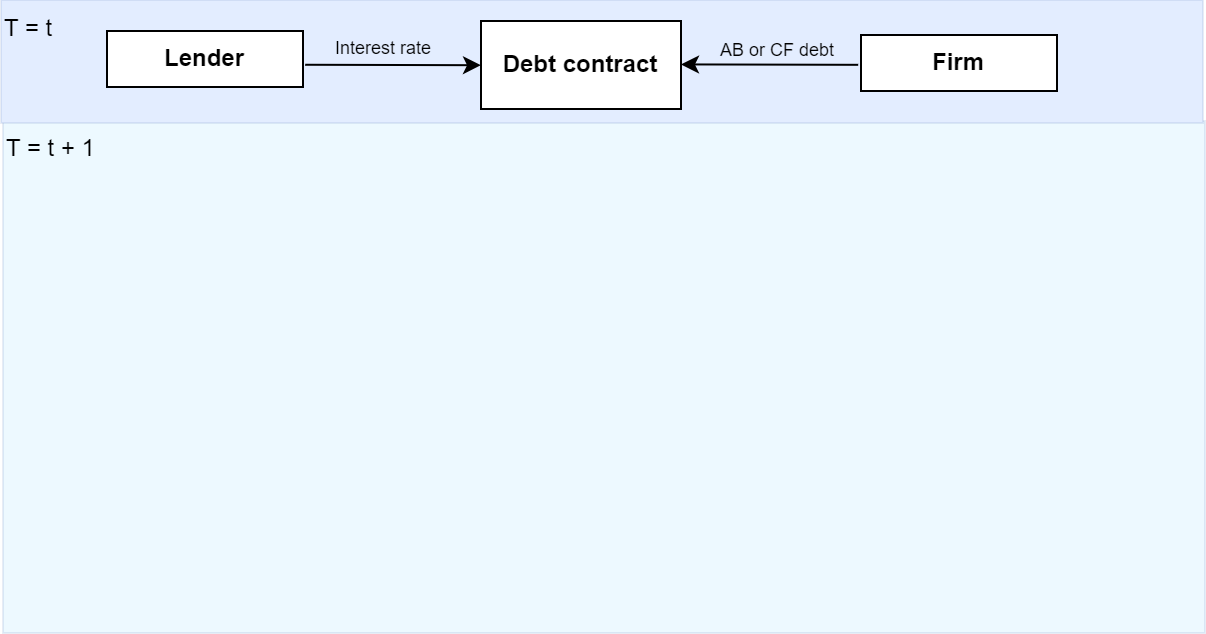
\includegraphics[width=0.95\textwidth]{Plots/min60_t1.png}}
\only<2>{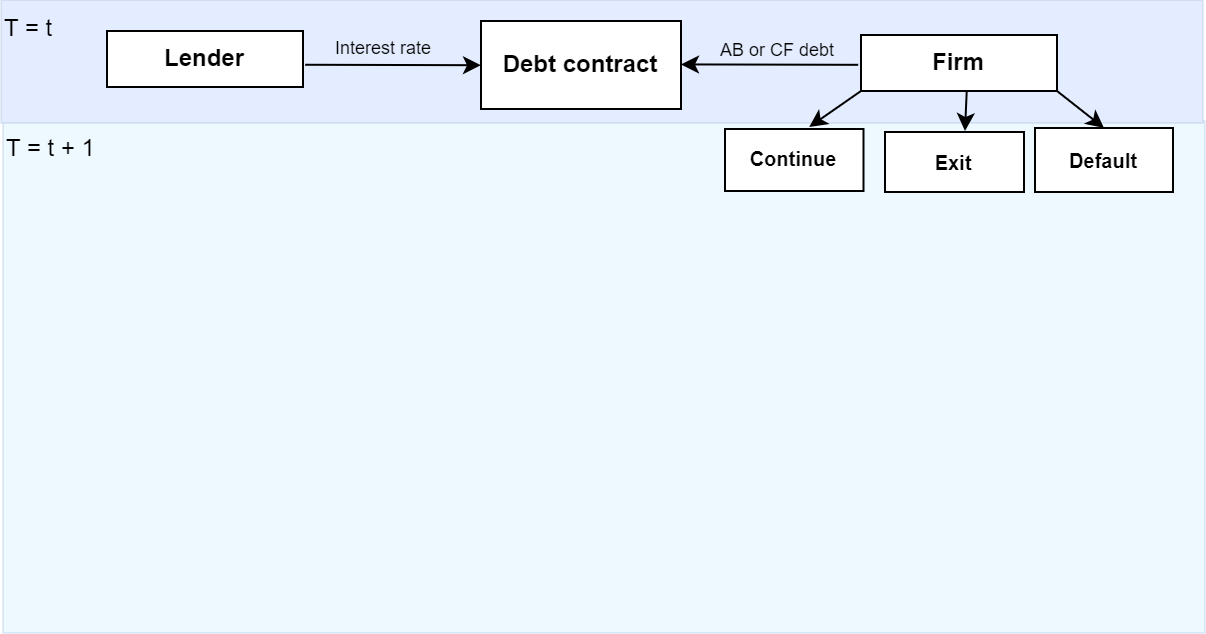
\includegraphics[width=0.95\textwidth]{Plots/min60_t2.png}}
\only<3>{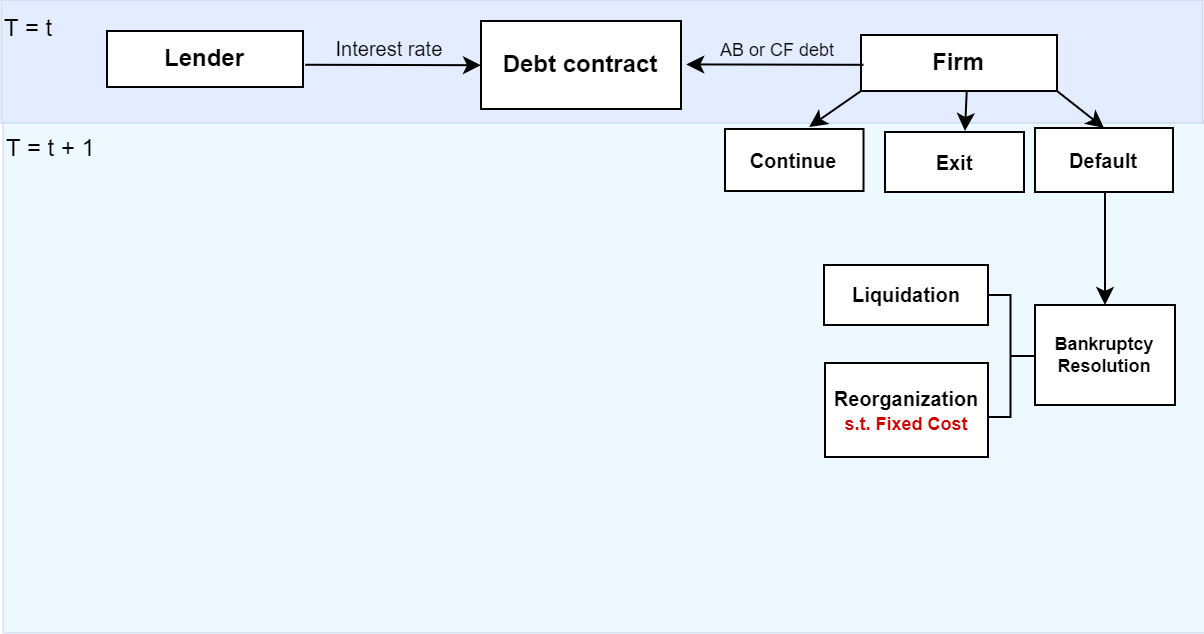
\includegraphics[width=0.95\textwidth]{Plots/min60_t4_fc.png}}
\only<4>{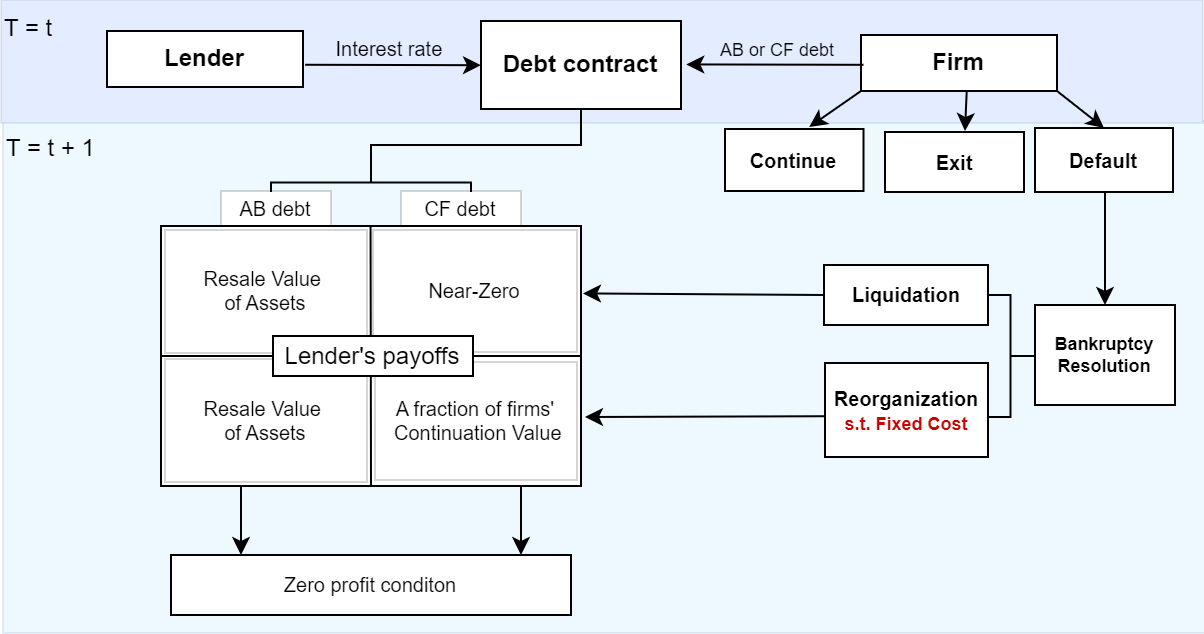
\includegraphics[width=0.95\textwidth]{Plots/min60_t6_fc.png}}
\only<5>{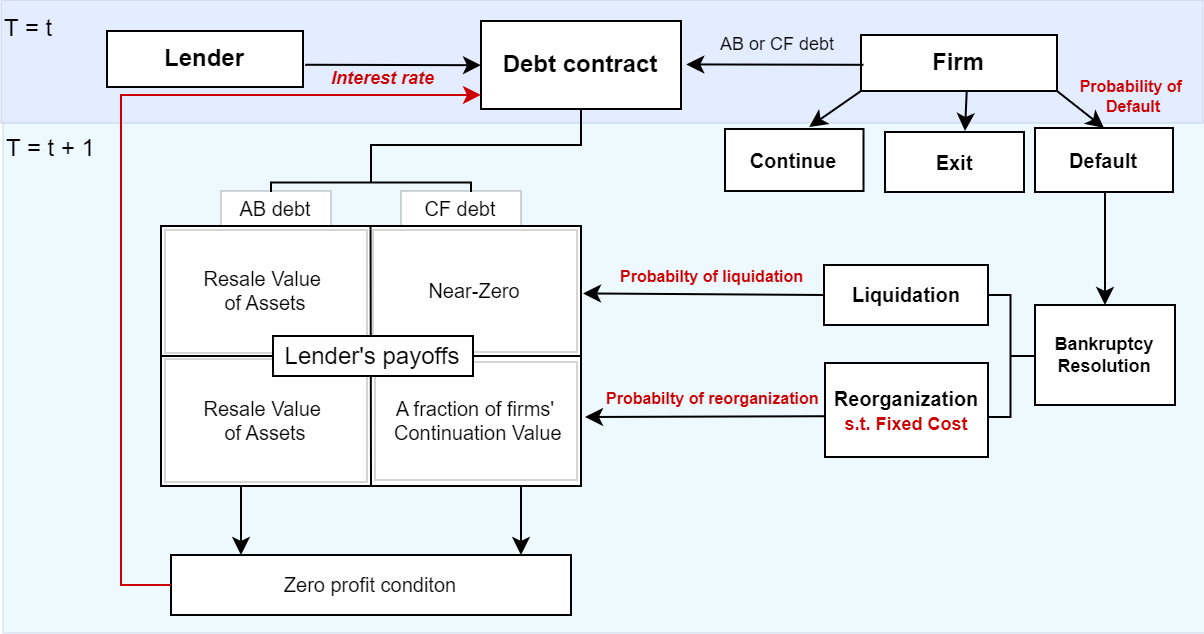
\includegraphics[width=0.95\textwidth]{Plots/min60_t7_fc.png}}

\end{frame}

%----------------------------------------------------------------------------------------
%	SLIDE 4 -- EFFECTS  (firm-level + aggregate in one table) + bullets
%----------------------------------------------------------------------------------------
\begin{frame}[label=effects] \frametitle{Main Results -- Cutting Reorganization Costs \hfill \hyperlink{modelfit}{\beamergotobutton{Calibration}}}

\textbf{Experiment:} cut the fixed reorganization cost by half
\begin{itemize} \small
    \item Average liquidation probability falls from $\sim 56\%$ to $\sim 39\%$
\end{itemize} \normalsize \vspace{1mm}

\begin{columns}[T,onlytextwidth]
\begin{column}{0.57\textwidth}
\centering \footnotesize
\textbf{Firm-level} \;{\scriptsize(Baseline $\to$ \textcolor{primary}{Reform})}\\[1mm]
\renewcommand{\arraystretch}{0.95}
\begin{tabular}{lcc}
\toprule
 & \textbf{Small} & \textbf{Large} \\
\midrule
Pr. Liquidation & 0.86\,$\to$\,\textcolor{primary}{0.63} & 0.14\,$\to$\,\textcolor{primary}{0.03} \\
Debt/Collateral & 0.45\,$\to$\,\textcolor{primary}{0.48} & 0.57\,$\to$\,\textcolor{primary}{0.57} \\
Interest Rate   & 5.63\,$\to$\,\textcolor{primary}{5.23} & 4.89\,$\to$\,\textcolor{primary}{4.63} \\
CF Reliance     & 0.24\,$\to$\,\textcolor{primary}{0.43} & 0.97\,$\to$\,\textcolor{primary}{0.99} \\
\bottomrule
\end{tabular}
\end{column}
\begin{column}{0.42\textwidth}
\centering \footnotesize
\textbf{Aggregate}\\[1mm]
\renewcommand{\arraystretch}{0.95}
\begin{tabular}{lccc}
\toprule
 & \textbf{Base} & \textbf{Ref.} & \textbf{\%$\Delta$} \\
\midrule
No.\ Firms & 10.00 & 10.71 & +7.10\% \\
$K/L$ & 3.42 & 3.52 & +2.92\% \\
Prod.\ $(Y/L)$ & 2.00 & 2.035 & \textcolor{primary}{+1.75\%} \\
\bottomrule
\end{tabular}
\end{column}
\end{columns}
\vspace{4mm}

\begin{itemize} \small
    \item Small firms benefit from lower liquidation risk and cheaper external finance
    \item Lower financing frictions raise capital intensity and increase firm entry
\end{itemize}
Productivity gains are driven by an increased mass of small and middle-market firms

\end{frame}

 
%----------------------------------------------------------------------------------------
%	SLIDE 5  -- CONCLUSIONS  
%----------------------------------------------------------------------------------------
\begin{frame}[label=conclusions2] \frametitle{Conclusions}
 
High ex-ante liquidation risk is a major impediment to small firms' access to credit \vspace{3mm}

Facilitating reorganization improves credit allocation and productivity. 
\begin{itemize} \small
    \item Cutting liquidation risk by 17 pp.\ improves aggregate productivity by 1.75\%
\end{itemize} \normalsize \vspace{5mm}

 
Bankruptcy reforms improve credit allocation and productivity \vspace{-4mm}
 
\begin{columns}[T,onlytextwidth]
\begin{column}{0.47\textwidth}
\begin{tcolorbox}[colback=lightblue,colframe=primary,boxrule=1pt,arc=1.5mm,left=2mm,right=2mm,top=0.8mm,bottom=0.8mm,halign=center]
\small \textbf{\textcolor{primary}{SBRA}} (U.S., 2020)
\end{tcolorbox}
\end{column}
\begin{column}{0.47\textwidth}
\begin{tcolorbox}[colback=lightblue,colframe=primary,boxrule=1pt,arc=1.5mm,left=2mm,right=2mm,top=0.8mm,bottom=0.8mm,halign=center]
\small \textbf{\textcolor{primary}{EU Reorg.\ Directive}} (2019)
\end{tcolorbox}
\end{column}
\end{columns}   \vspace{3mm}
\begin{itemize}
    \item Both reforms streamline reorganization and cut administrative costs
    \item Applied to the SBRA, the model implies a \textbf{\textcolor{primary}{0.81\% gain}} in aggregate productivity
\end{itemize} \normalsize
 
\end{frame}

%----------------------------------------------------------------------------------------
%	APPENDIX -- EMPIRICAL MOTIVATION (target of the slide-1 hyperlink)
%----------------------------------------------------------------------------------------
\appendix

\begin{frame}[label=empirics] \frametitle{Empirical Motivation \hfill \hyperlink{motivation}{\beamergotobutton{Back}}}

Cash flow-based debt is expensive for smaller firms
\footnotesize
\begin{table}[h]
    \centering
    \renewcommand{\arraystretch}{1}
    \begin{tabular}{lcc}
        \toprule
        \textbf{Credit Spread} & \textbf{$\leq$ 100M USD} & \textbf{$>$ 100M USD} \\
        \midrule
        Cash flow-based debt & 7.19\% & 3.12\% \\
        Asset-based debt     & 5.25\% & 3.93\% \\
        \bottomrule
        & \multicolumn{2}{r}{\textit{\scriptsize Source: Compustat, CapitalIQ}} \\
    \end{tabular}
\end{table}
\normalsize \vspace{2mm}

Liquidation risk is substantial for smaller firms
\footnotesize
\begin{table}[h]
    \centering
    \renewcommand{\arraystretch}{1}
    \begin{tabular}{lcc}
        \toprule
        \textbf{Liquidation Risk} & \textbf{$\leq$ 100M USD} & \textbf{$>$ 100M USD} \\
        \midrule
        Share Liquidated & 76.7\% & 7.61\% \\
        \bottomrule
        & \multicolumn{2}{r}{\textit{\scriptsize Source: FJC Integrated Database}} \\
    \end{tabular}
\end{table}
\normalsize

\end{frame}

%----------------------------------------------------------------------------------------
%	BACKUP -- MODEL FIT (target of the main-results "motivation" hyperlink)
%----------------------------------------------------------------------------------------
\begin{frame}[label=modelfit] \frametitle{Model Fit \hfill \hyperlink{effects}{\beamergotobutton{Back}}}

\textbf{Targeted moments} based on U.S.\ non-financial corporations, 2010--2024
\begin{itemize} \small
    \item Model closely matches liquidation risk and firms' debt financing choices
\end{itemize} \normalsize \vspace{1mm}

\footnotesize
\begin{table}[h!]
\centering
\renewcommand{\arraystretch}{0.85}
\begin{tabular}{l|cc||cc}
& \multicolumn{2}{c||}{\textbf{Targeted}} & \multicolumn{2}{c}{\textbf{Untargeted} (Data -- \textcolor{primary}{Model})} \\
\toprule
\textbf{Moment} & \textbf{Target} & \textbf{Model} & \textbf{Small} & \textbf{Large} \\
\midrule
Liquidation prob.   & 0.58 & \textcolor{primary}{0.56} & 0.84 -- \textcolor{primary}{0.85} & 0.20 -- \textcolor{primary}{0.14} \\
Debt/Collateral     & 0.52 & \textcolor{primary}{0.50} & 0.44 -- \textcolor{primary}{0.45} & 0.59 -- \textcolor{primary}{0.57} \\
Interest rate       & 5.36 & \textcolor{primary}{5.30} & 5.89 -- \textcolor{primary}{5.63} & 4.63 -- \textcolor{primary}{4.89} \\
CF-reliance         & 0.51 & \textcolor{primary}{0.53} & 0.51 -- \textcolor{primary}{0.24} & 0.53 -- \textcolor{primary}{0.97} \\
CF debt/total debt  & 0.82 & \textcolor{primary}{0.82} & 0.34 -- \textcolor{primary}{0.30} & 0.83 -- \textcolor{primary}{0.87} \\
\bottomrule
\end{tabular}
\label{tab:model_fit}
\end{table}
\normalsize \vspace{1mm}

\begin{itemize} \small
    \item Captures the higher liquidation risk and financing gap faced by small firms
    \item Reproduces the stronger reliance on cash flow-based debt among large firms
\end{itemize}

\end{frame}

\end{document}